\documentclass{article}
\usepackage{graphicx} % Required for inserting images
\usepackage[nonumberlist]{glossaries}
\usepackage[italian]{babel}
\usepackage{hyperref}
\usepackage[noabbrev]{cleveref}
\usepackage{biblatex}
\usepackage[margin=1in]{geometry}
\usepackage{forest}

\definecolor{folderbg}{RGB}{124,166,198}
\definecolor{folderborder}{RGB}{110,144,169}

\def\Size{4pt}
\tikzset{
      folder/.pic={
        \filldraw[draw=folderborder,top color=folderbg!50,bottom color=folderbg]
          (-1.05*\Size,0.2\Size+5pt) rectangle ++(.75*\Size,-0.2\Size-5pt);  
        \filldraw[draw=folderborder,top color=folderbg!50,bottom color=folderbg]
          (-1.15*\Size,-\Size) rectangle (1.15*\Size,\Size);
      }
    }

\crefformat{section}{\S#2#1#3}
\crefformat{subsection}{\S#2#1#3}
\crefformat{subsubsection}{\S#2#1#3}
\crefformat{figure}{#2Figura~#1#3}
\crefformat{footnote}{#2\footnotemark[#1]#3}
\crefformat{table}{#2Tabella~#1#3}
\crefformat{equation}{#2Equazione~#1#3}
\crefformat{chapter}{#2Capitolo~#1#3}

\addbibresource{refs.bib}

\renewcommand{\contentsname}{Indice}

\makeglossaries

\newglossaryentry{player} 
{  
    name={player (\textmd{oppure} giocatore)},
    text=giocatore,
    description=è l'entità che può eseguire un turno nei round di un game. Un player può essere umano o un robot
}

\newglossaryentry{game}
{
    name={game (\textmd{oppure} gioco, partita)},
    text=partita,
    description={è l'entità principale del sistema. Un game è composto da più round}
}

\newglossaryentry{round}
{
    name=round,
    text=round,
    description={è l'entità che contiene le informazioni di gioco principali. Ogni game è composto da un numero 
    finito di round durante il quale ciascun giocatore effettua la propria giocata}
}

\newglossaryentry{turn}
{
    name={turn (\textmd{oppure} turno)},
    text=turno,
    description={è l'unità indivisibile di un round e rappresenta le azioni di un giocatore durante il round. Quindi contiene informazioni sull'esito dell'esecuzione dei test ed i relativi 
    risultati nonché le classi generate per risolvere il problema}
}

\begin{document}

\begin{titlepage}
    \begin{center}
        \vspace*{1cm}
            
        \Huge
        \textbf{Software Architecture Design}
            
        \vspace{0.5cm}
        \LARGE
        Game Repository - Iterazione 2
        
        \vfill
        \vspace{0.8cm}
        
        \Large
        Angelino Pasquale - M63001481 \\
        Capasso Giuseppe -  M63001498 \\
        Dinetti Andrea -  M63001496

    \end{center}
\end{titlepage}

\thispagestyle{empty}

\printglossaries

\newpage
\thispagestyle{empty}
\tableofcontents

\newpage
\thispagestyle{empty}
\section*{Introduzione}
In questa sezione, sarà effettuata una breve descrizione del progetto focalizzandosi sul \textit{task} assegnato.\\ 

L'attività assegnata prevede la progettazione e implementazione del componente \textit{Game Repository} che 
si occupa di memorizzare, per ogni \gls{game} giocata, informazioni quali il tipo, i \gls{round} giocati, 
le classi di test prodotte dai giocatori.\\

Il gruppo si coordina e gestisce le proprie attività con questo progetto
(consultabile al seguente \href{https://github.com/users/alarmfox/projects/2}{link}) in linea con le metodologie di sviluppo AGILE.

\newpage
\section{Attività svolte}
In questa sezione, saranno presentate le attività svolte.

\subsection{Completamento CRUD API per \textit{game}, \textit{round}, \textit{turni}}
Sono state implementate le funzionalità CRUD per le entità descritta durante la fase di ideazione.
In particolare, l'utente può effettuare l'aggiornamento di una partita come mostrato in \cref{fig:upd_game}. 

\begin{figure}[h]
    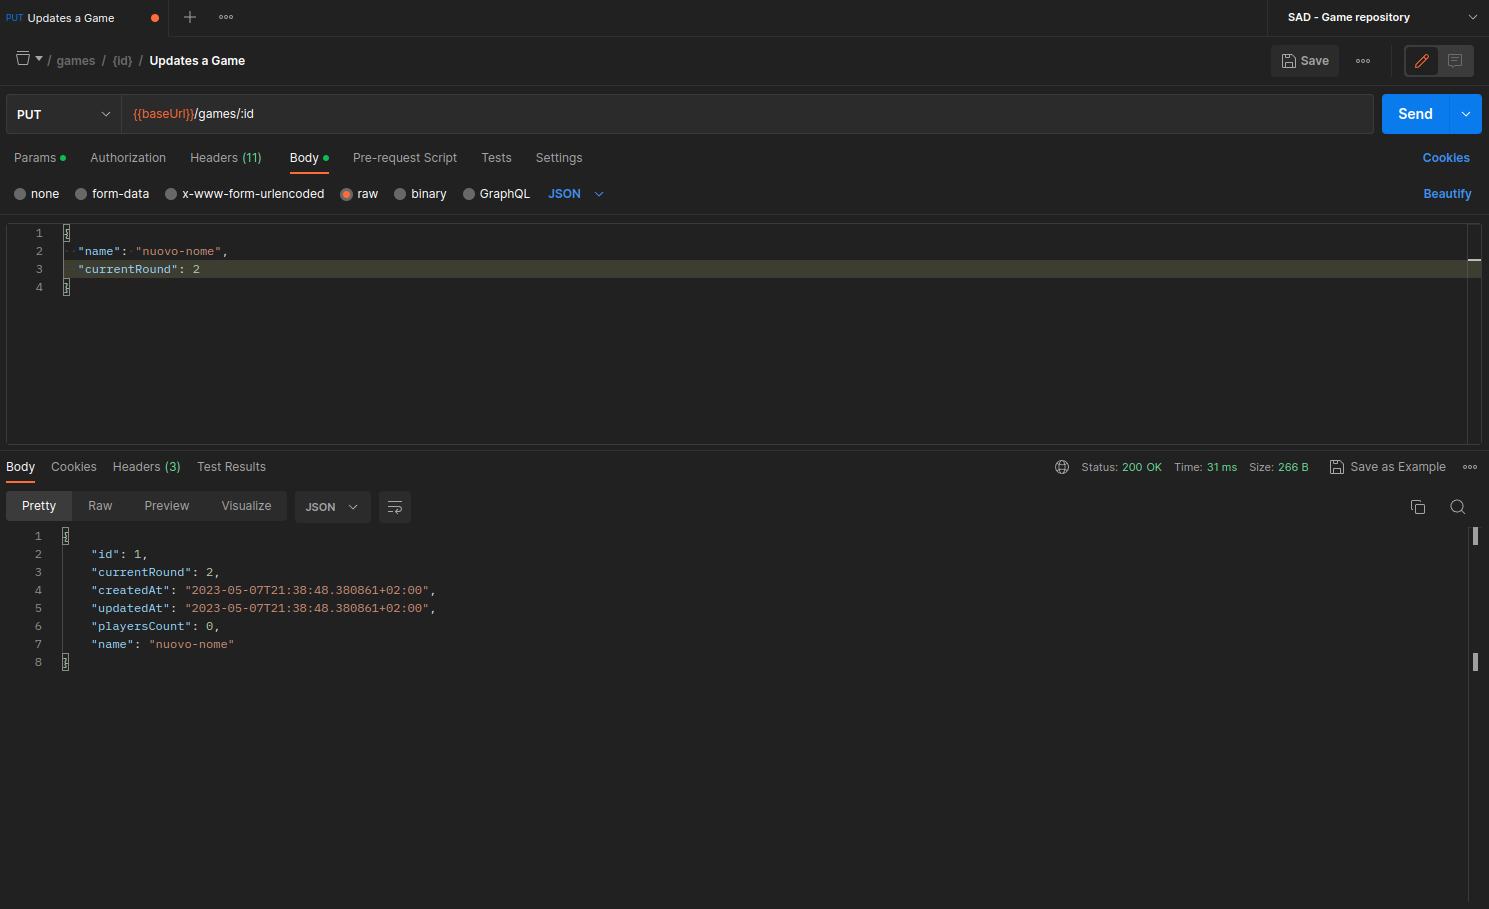
\includegraphics[width=\textwidth]{images/upd_game.png}
    \caption{Aggiornamento di una partita}
    \label{fig:upd_game}
\end{figure}

Inoltre, adesso è possibile eseguire le operazioni di CRUD sui round, come mostrato in \cref{fig:cr_round} e \cref{fig:get_round}.

\begin{figure}
    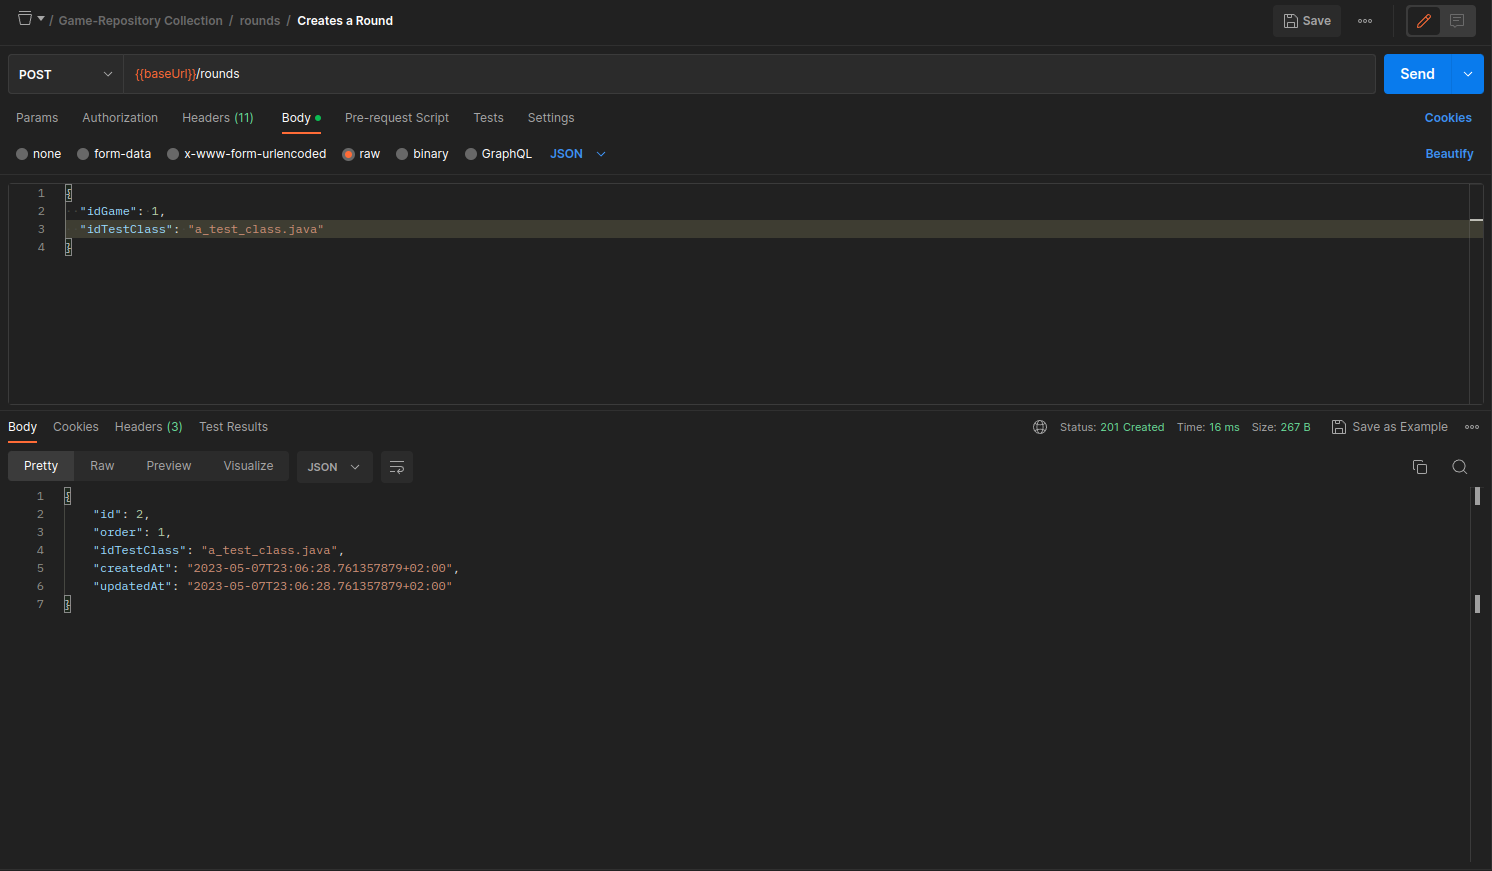
\includegraphics[width=\textwidth]{images/cr_round.png}
    \caption{Creazione di un round}
    \label{fig:cr_round}
\end{figure}

\begin{figure}
    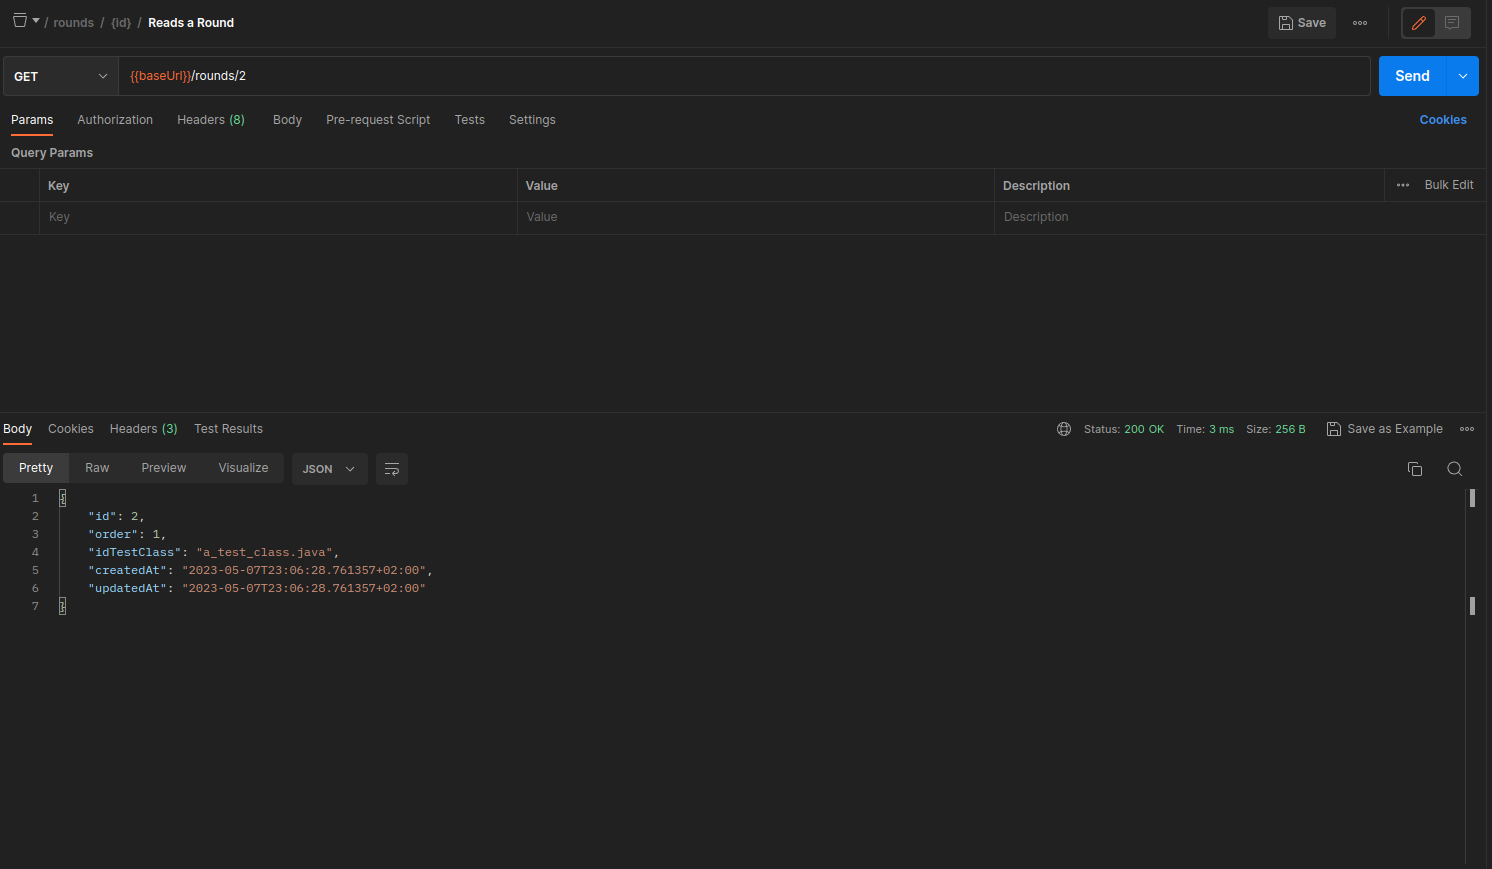
\includegraphics[width=\textwidth]{images/get_round.png}
    \caption{Recupero di un round}
    \label{fig:get_round}
\end{figure}

\clearpage
\subsection{Implementazione salvataggio e recupero dei file prodotti dagli utenti}
Il sistema implementato accetta uno \textit{zip} contente tutti i file prodotti dagli utenti che
sarà salvato in una gerarchia di cartelle strutturata come mostarto di seguito. Inoltre, è possibile per l'utente configurare la posizione della cartella \textit{root}.

 \begin{forest}
      for tree={
        font=\ttfamily,
        grow'=0,
        child anchor=west,
        parent anchor=south,
        anchor=west,
        calign=first,
        inner xsep=7pt,
        edge path={
          \noexpand\path [draw, \forestoption{edge}]
          (!u.south west) +(7.5pt,0) |- (.child anchor) pic {folder} \forestoption{edge label};
        },
        % style for your file node 
        file/.style={edge path={\noexpand\path [draw, \forestoption{edge}]
          (!u.south west) +(7.5pt,0) |- (.child anchor) \forestoption{edge label};},
          inner xsep=2pt,font=\small\ttfamily
                     },
        before typesetting nodes={
          if n=1
            {insert before={[,phantom]}}
            {}
        },
        fit=band,
        before computing xy={l=15pt},
      }  
    [data
      [\textit{ANNO}
       [\textit{ID-GAME}
        [1.zip
        ]
        [2.zip
        ]
        [3.zip
        ]
      ]
      [\textit{ID-GAME}
        [4.zip
        ]
        [5.zip
        ]
        [6.zip
        ]
      ]
      ]
       [\textit{ANNO}
       [\textit{ID-GAME}
        [11.zip
        ]
        [12.zip
        ]
        [13.zip
        ]
      ]
      [\textit{ID-GAME}
        [14.zip
        ]
        [15.zip
        ]
        [16.zip
        ]
      ]
      ]
    ]
 \end{forest}
\clearpage

\subsection{Implementazione CI}
Attraverso le Github Actions, è stato predisposto un sistema minimale di Continuous Integration in cui il \textit{branch master} è protetto dall'esecuzione di test per le funzionalità principali dell'applicazione. Inoltre, è stato protetto il \textit{branch master} dal \textit{push} diretto avendo così sempre una versione stabile integrata solo attraverso le \textit{pull request} che superano i test. La presenza delle Github Actions offre informazioni sullo stato della \textit{build}, come mostrato in \cref{fig:ci}.

\begin{figure}[h]
    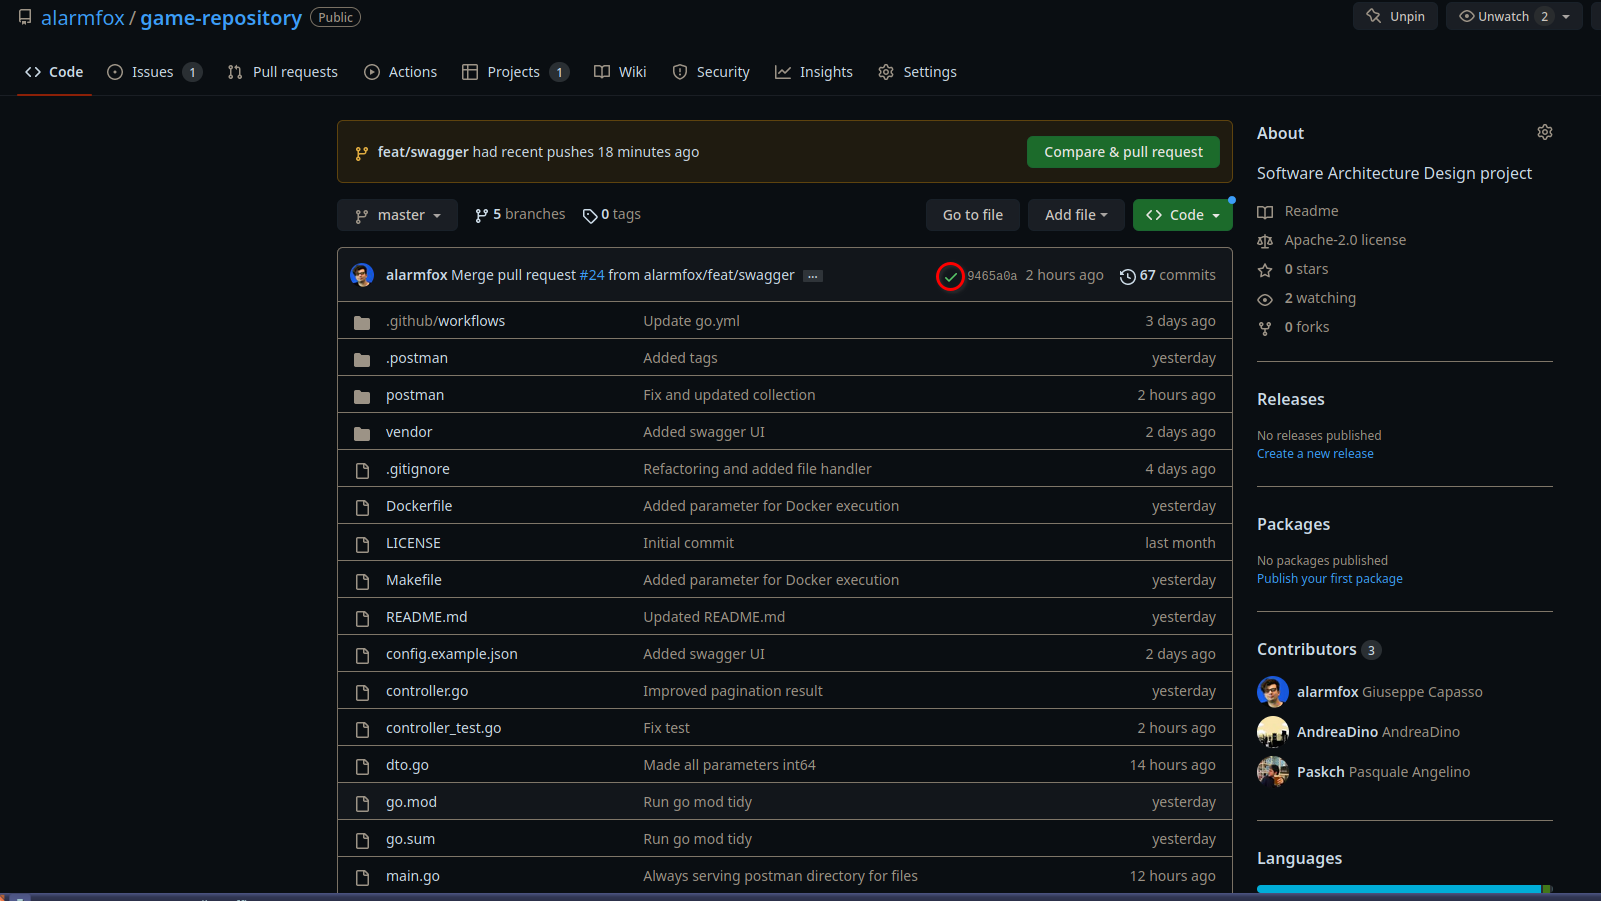
\includegraphics[width=\textwidth]{images/ci.png}
    \caption{Ricerca dei Game dall'inizio dell'anno con paginazione}
    \label{fig:ci}
\end{figure}

\clearpage

\subsection{Implementazione specifica OpenAPI e Swagger UI}
Attraverso Postman è stata progettata la specifica OpenAPI degli endpoint ed è stata integrata attraverso github sul progetto principale. Inoltre, dalla specifica è stata generata automaticamente una collection per facilitare il testing e l'integrazione del Game Repository da parte degli utenti. Infine, è stata effettuata un'integrazione all'interno del progetto per esporre una \textit{Swagger UI} e servire sia la specifica OpenAPI che la collection Postman quando l'applicazione viene configurata con il \textit{flag} \textbf{\textit{enableSwagger}} a \textit{True} (come mostrato in \cref{fig:swagger}).

\begin{figure}[h]
    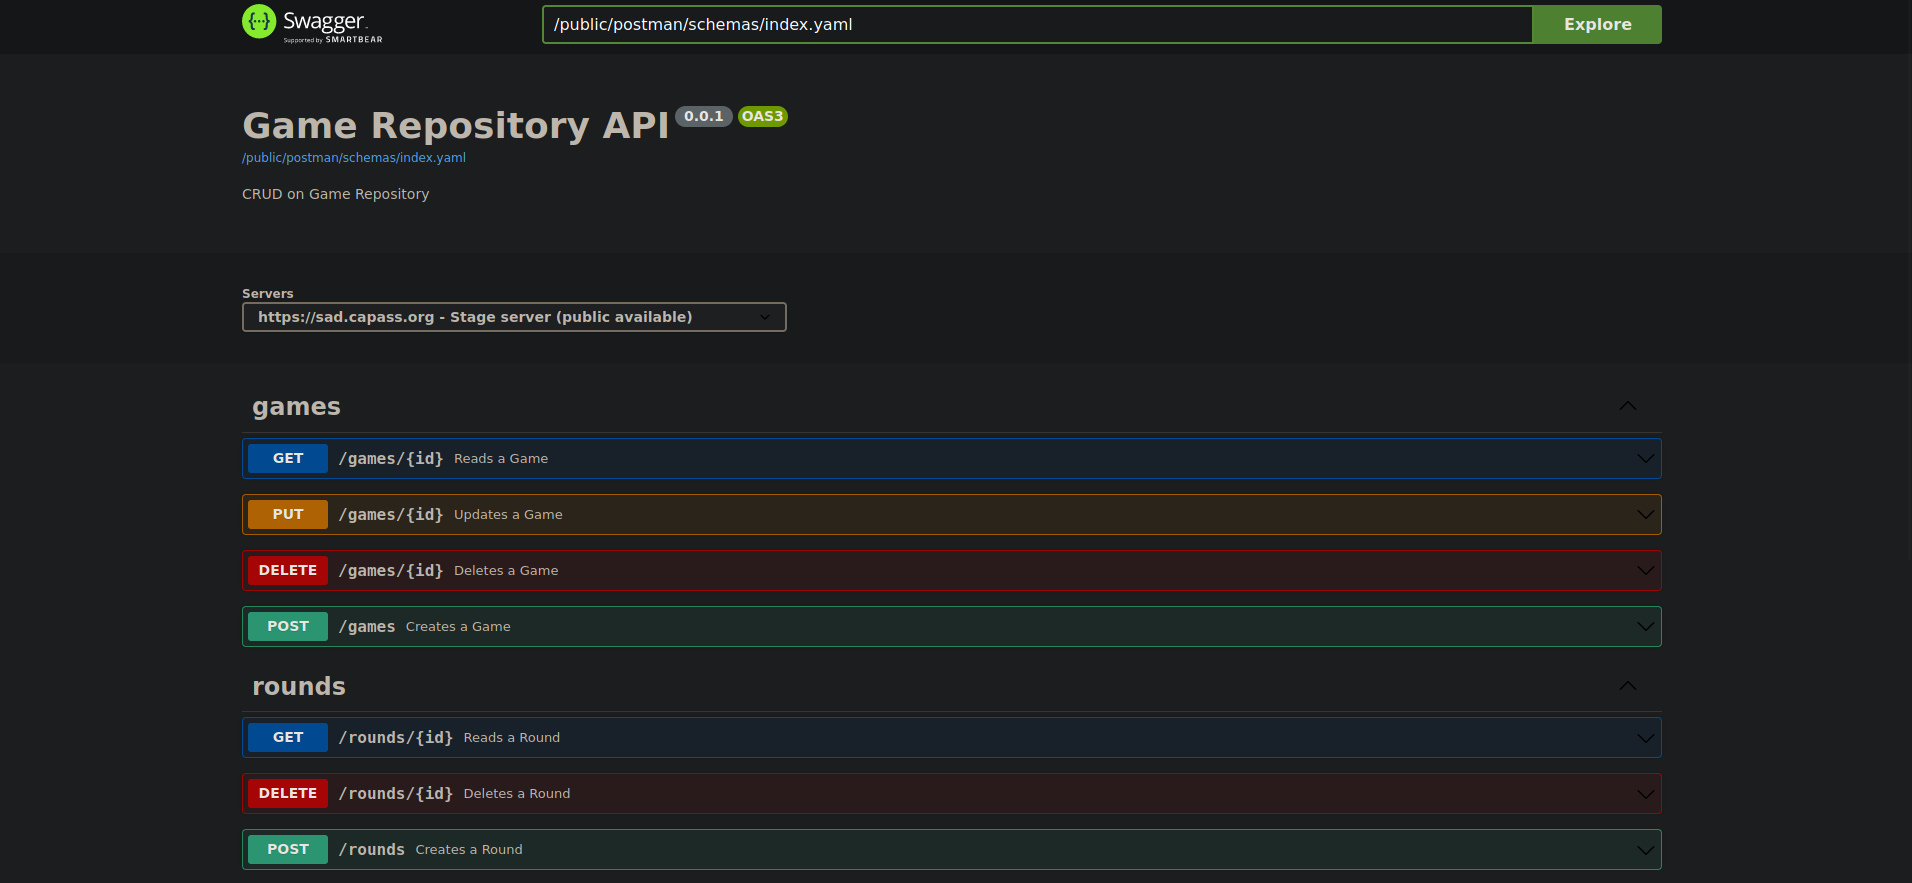
\includegraphics[width=\textwidth]{images/swagger.png}
    \caption{Swagger UI}
    \label{fig:swagger}
\end{figure}

\clearpage

\subsection{Implementazione delle operazioni di \textit{list}}
\paragraph{List delle partite} Per le partite è possibile effettuare le operazioni di list per intervallo temporale con supporto alla paginazione. In \cref{fig:list_game}, è mostrata una richiesta per avere le partite dell'ultimo anno con pagine di 50 elementi ciascuno.

\begin{figure}[h]
    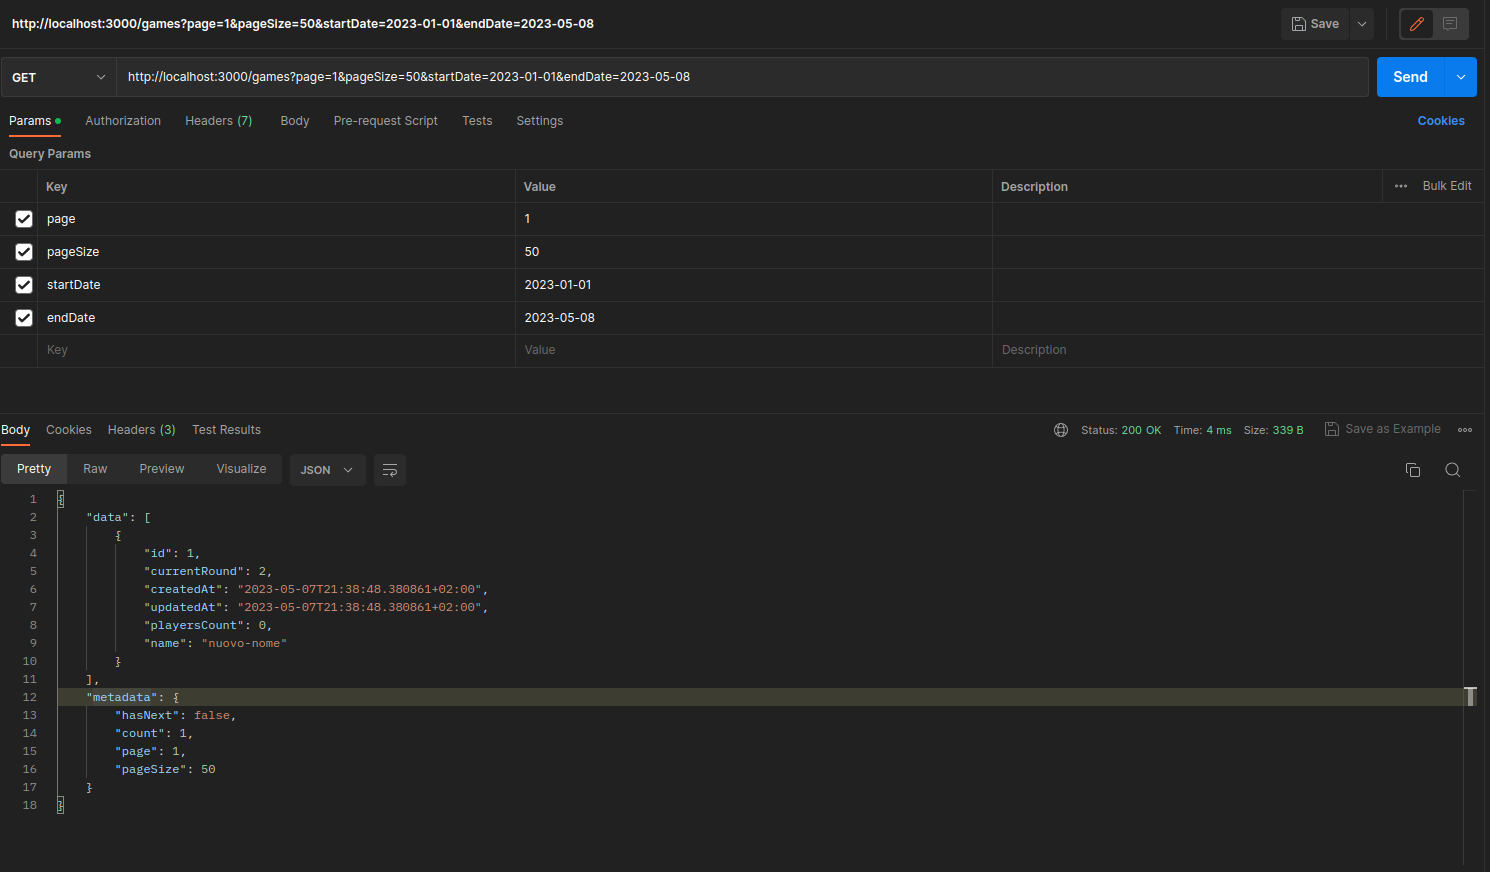
\includegraphics[width=\textwidth]{images/list_game.png}
    \caption{Ricerca dei Game dall'inizio dell'anno con paginazione}
    \label{fig:list_game}
\end{figure}

\paragraph{List dei round}
È possibile recuperare tutti i round di una partita, come mostrato in \cref{fig:list_round}.

\begin{figure}[h]
    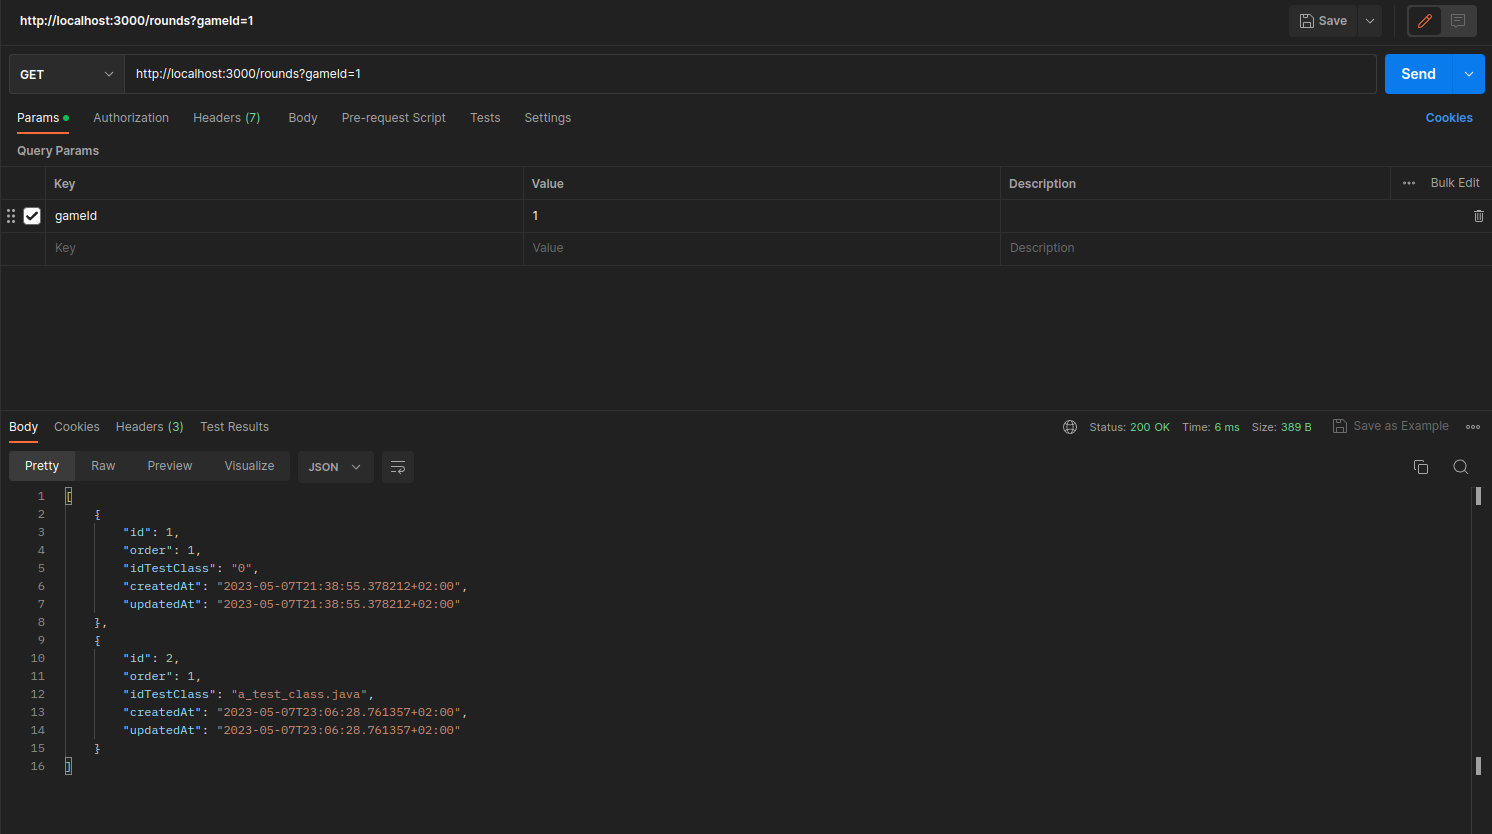
\includegraphics[width=\textwidth]{images/list_round.png}
    \caption{Ricerca dei round all'interno di una partita}
    \label{fig:list_round}
\end{figure}

\paragraph{List dei turni}
È possibile recuperare tutti i turni di un round, come mostrato in \cref{fig:list_turn}.

\begin{figure}[h]
    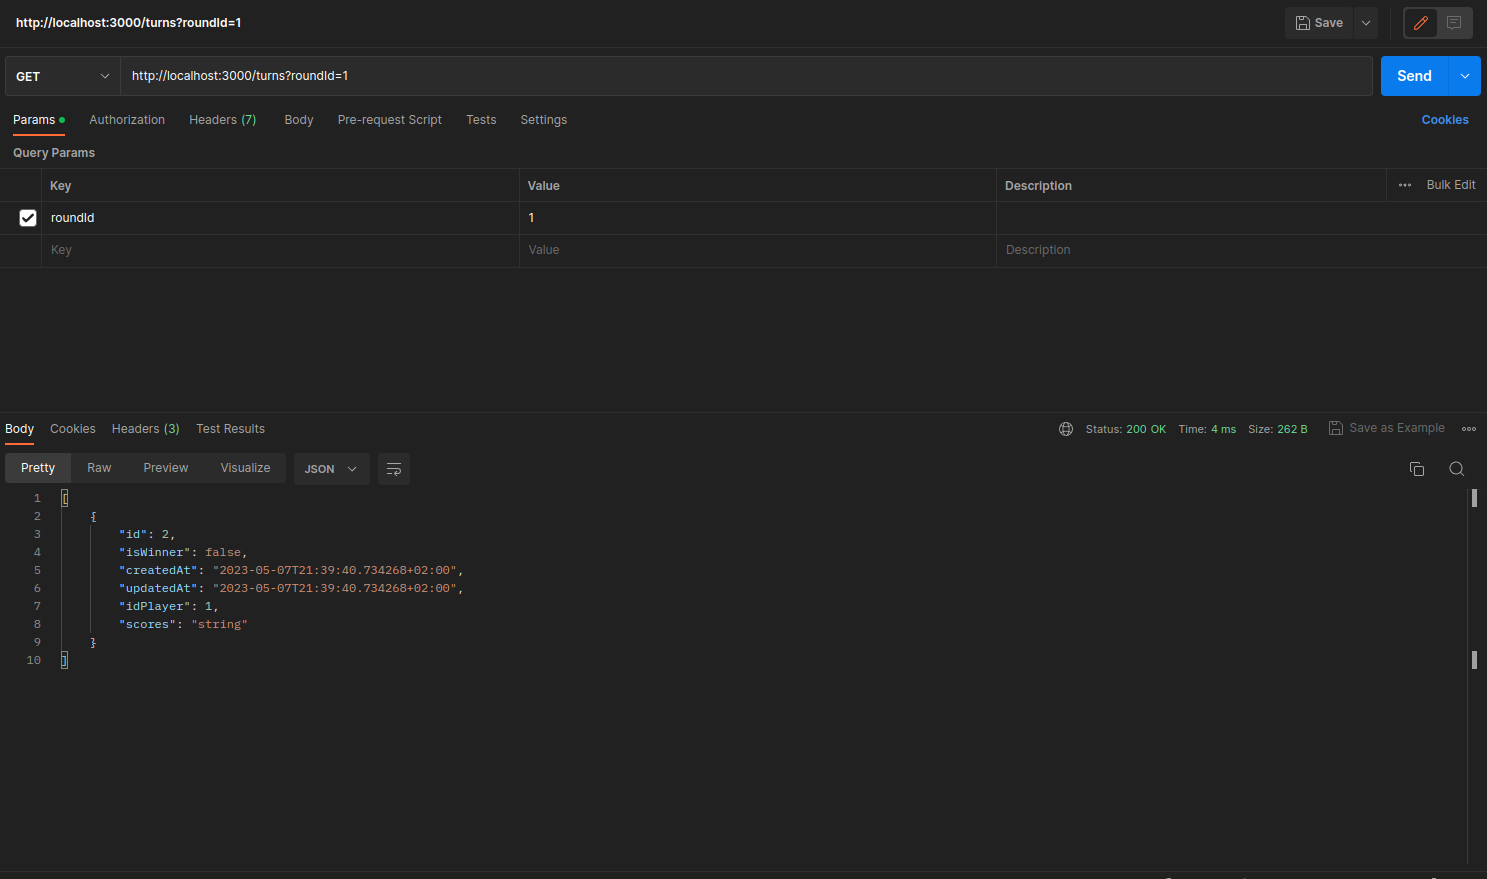
\includegraphics[width=\textwidth]{images/list_turn.png}
    \caption{Ricerca dei turni all'interno di un round}
    \label{fig:list_turn}
\end{figure}

\clearpage
\section{Conclusione e pianificazione prossima iterazione}
L'attività si conclude con il \textit{deploy} manuale su questo \href{https://sad.capass.org}{URL} del prototipo funzionante. In particolare, navigando \href{https://sad.capass.org/docs} {qui} è possibile accedere alla Swagger UI e provare gli endpoint implementati.\\

Nella \cref{tab:next_phase} sono elencate le attività da svolgere nella fase successiva.


\begin{table}[h]
    \centering
    \begin{tabular}{|l|p{0.4\linewidth}|}
        \hline
         Attività & Descrizione \\
        \hline
        \hline
         Analisi review & Eventuale modifica dell'architettura in base alla review. \\
        \hline
        Integrazione prototipo & Aggiunta delle proprietà relative al modello ER nelle API CRUD implementate. \\ 
        \hline
        Gestione bot & Gestione separata degli utenti umani da quelli robot. \\ 
        \hline
        Continous Deployment & Progettazione delle attività per produrre automaticamente eseguibili e/o immagini Docker. \\
        \hline
        Cursor based pagination & Analisi della paginazione \textit{cursor based} per sostituire quella "\textit{skip and limit}".\\
        \hline
    \end{tabular}
    \caption{Pianificazione attività per prossima fase}
    \label{tab:next_phase}
\end{table}


\clearpage

\printbibliography

\end{document}